\documentclass{beamer}
\usepackage{ctex, hyperref}
%\usepackage[T1]{fontenc}
\usepackage{amsfonts,amsmath,oldgerm}
\usetheme{sintef}


\newcommand{\testcolor}[1]{\colorbox{#1}{\textcolor{#1}{test}}~\texttt{#1}}

\usefonttheme[onlymath]{serif}

\titlebackground*{assets/background}

\newcommand{\hrefcol}[2]{\textcolor{cyan}{\href{#1}{#2}}}

\title{Calculus}
\course{2023牛剑营数学}
\author{唐业腾}

\begin{document}
\maketitle
\CJKfamily{zhkai}

\section{Limit}
\begin{frame}{Definition}
Formally, the definition of the "limit of $f(x)$ as $x$ approaches $c$ " is given as follows. The limit is a real number $L$ so that, given an arbitrary real number $\epsilon>0$ (thought of as the "error"), there is a $\delta>0$ such that, for any $x$ satisfying $0<|x-c|<\delta$, it holds that $|f(x)-L|<\epsilon$. This is known as the $(\epsilon, \delta)$-definition of limit.\\
Note:\\
(a) It is possible to define the notion of "tending to infinity" in the domain of $f$,
$$
\lim _{x \rightarrow \infty} f(x)=L .
$$
In this expression, the infinity is considered to be signed: either $+\infty$ or $-\infty$.\\
(b) It is also possible to define the notion of "tending to infinity" in the value of $f$,
$$
\lim _{x \rightarrow c} f(x)=\infty
$$
\end{frame}

\begin{frame}{One-sided vs. two-sided}
    It is possible to define the notion of having a "left-handed" limit ("from below"), and a notion of a "right-handed" limit ("from above"). These need not agree.\\
    For example, $f: \mathbb{R} \rightarrow \mathbb{R}$, defined such that $f(x)=0$ if $x \leq 0$, and $f(x)=1$ if $x>0$. At $x=0$, $\lim _{x \rightarrow 0^{-}} f(x)=0$, and $\lim _{x \rightarrow 0^{+}} f(x)=1$, and from this it can be deduced $\lim _{x \rightarrow 0} f(x)$ doesn't exist, because $\lim _{x \rightarrow 0^{-}} f(x) \neq \lim _{x \rightarrow 0^{+}} f(x)$.
\end{frame}

\begin{frame}{Theorems on limits}
    \begin{itemize}
        \item $\lim _{x \rightarrow c}[kf(x)]=k\lim _{x \rightarrow c} f(x)$, where $k$ is a constant
        \item $\lim _{x \rightarrow c}[f(x) \pm g(x)]=\lim _{x \rightarrow c} f(x) \pm \lim _{x \rightarrow c} g(x)$
        \item $\lim _{x \rightarrow c}[f(x) g(x)]=\lim _{x \rightarrow c} f(x) \cdot \lim _{x \rightarrow c} g(x)$
        \item $\lim _{x \rightarrow c}\left[\frac{f(x)}{g(x)}\right]=\frac{\lim _{x \rightarrow c} f(x)}{\lim _{x \rightarrow c} g(x)}$, provided $\lim _{x \rightarrow c} g(x) \neq 0$
    \end{itemize}
\end{frame}

\begin{frame}{Useful results for limits}
    \begin{itemize}
        \item $\lim _{x \rightarrow a}c=c$, where $c$ is a constant
        \item $\lim _{x \rightarrow +\infty}\frac{1}{x^n}=0$, $n\in \mathbb{R}$
        \item $\lim _{x \rightarrow -\infty}\frac{1}{x^n}=0$, $n\in \mathbb{R}$
        \item $\lim _{n \rightarrow+\infty}\left(1+\frac{1}{n}\right)^n=e$
        \item $\lim _{x \rightarrow 0} \frac{\sin x}{x}=1$
    \end{itemize}
\end{frame}

\begin{frame}{L'Hôpital's rule}
    L'Hôpital's rule states that for functions $f$ and $g$ which are differentiable on an open interval $I$ except possibly at a point $c$ contained in $I$, if $\lim _{x \rightarrow c} f(x)=\lim _{x \rightarrow c} g(x)=0$ or $\pm \infty$, and $g^{\prime}(x) \neq 0$ for all $x$ in $I$ with $x \neq c$, and $\lim _{x \rightarrow c} \frac{f^{\prime}(x)}{g^{\prime}(x)}$ exists, then
$$
\lim _{x \rightarrow c} \frac{f(x)}{g(x)}=\lim _{x \rightarrow c} \frac{f^{\prime}(x)}{g^{\prime}(x)} .
$$
The differentiation of the numerator and denominator often simplifies the quotient or converts it to a limit that can be evaluated directly.
\end{frame}

\begin{frame}{L'Hôpital's rule}
    All four conditions for L'Hôpital's rule are necessary:\\
1. Indeterminacy of form: $\lim _{x \rightarrow c} f(x)=\lim _{x \rightarrow c} g(x)=0$ or $\pm \infty$; and\\
2. Differentiability of functions: $f(x)$ and $g(x)$ are differentiable on an open interval $\mathcal{I}$ except possibly at a point $c$ contained in $\mathcal{I}$ (the same point from the limit) ; and\\
3. Non-zero derivative of denominator: $g^{\prime}(x) \neq 0$ for all $x$ in $\mathcal{I}$ with $x \neq c$; and\\
4. Existence of limit of the quotient of the derivatives: $\lim _{x \rightarrow c} \frac{f^{\prime}(x)}{g^{\prime}(x)}$ exists.
\end{frame}

\begin{frame}{Example 1}
Use L'Hôpital's rule to prove that $\lim _{x \rightarrow 0} \frac{\sin x}{x}=1$
\end{frame}

\begin{frame}{Example 2}
   Find $\lim _{x \rightarrow +\infty} \frac{x+\cos x}{x}$,you may use L'Hôpital's rule.\\
   How about $\lim _{x \rightarrow \infty} \frac{e^x+e^{-x}}{e^x-e^{-x}}$
\end{frame}

\section{Differentiation}
\begin{frame}{First principle of differentiation}
    We say a function $f$ is differentiable at a point $x_0$ if
$$
f^{\prime}\left(x_0\right)=\lim _{h \rightarrow 0} \frac{f\left(x_0+h\right)-f\left(x_0\right)}{h}
$$
exists. Also so we call $f^{\prime}\left(x_0\right)$ to be the derivative of $f$ at point $x_0$.
\end{frame}

\begin{frame}{Example 3}
     Use the first principle to derive the derivative of $x^n$. What are the possible cases to consider?
\end{frame}

\begin{frame}{Exercise 3}
    Use the first principle to derive the derivative of $sin(x)$ and $cos(x)$
\end{frame}

\begin{frame}{Example 4}
    Use the first principle to derive the derivative of $ln(x)$
\end{frame}

\begin{frame}{Example 5}
 Use the first principle to derive the product rule\\
 Let $h(x)=f(x) g(x)$.\\
Then $h^{\prime}(x)=f^{\prime}(x) g(x)+f(x) g^{\prime}(x)$
\end{frame}

\begin{frame}{Small "o" and big "O" notations}
    (i) " $f(x)=o(g(x))$ as $x \rightarrow x_0$ " if $\lim _{x \rightarrow x_0} \frac{f(x)}{g(x)}=0$. Intuitively, $f(x)$ is much smaller than $g(x)$.\\
    (ii) " $f(x)=O(g(x))$ as $x \rightarrow x_0$ " if $\frac{f(x)}{g(x)}$ is bounded as $x \rightarrow x_0$. Intuitively, $f(x)$ is about as big as $g(x)$.\\
    Note that for $f(x)=O(g(x))$ to be true, $\lim _{x \rightarrow x_0} \frac{f(x)}{g(x)}$ need not exist.\\
    Usually, $x_0$ is either 0 or infinity. Clearly, we have $f(x)=o(g(x))$ implies $f(x)=O(g(x))$\\
\end{frame}

\begin{frame}{Small "o" and big "O" notations}
For example\\
    $
    x \rightarrow \infty \\ 
    x^2+x=O\left(x^2\right) \quad  x^2=o\left(x^3\right) \\ 
    x \rightarrow 0 \\ 
    x^2+x=O(x) \quad  x^2=o(x)
    $
\end{frame}

\begin{frame}{Small "o" and big "O" notations}
For example\\
$\begin{aligned} & \sin x=x-\frac{x^3}{3 !}+\frac{x^5}{5 !}+O\left(x^7\right) \\ & \sin x=x-\frac{x^3}{3 !}+o\left(x^3\right)\end{aligned}$
\end{frame}

\begin{frame}{Example 6}
    (a) Prove that $f(x+h)=f(x)+h f^{\prime}(x)+o(h)$\\
    (b) Hence prove the Chain rule ($\frac{d y}{d x}=\frac{d y}{d u} \frac{d u}{d x}$)
\end{frame}

\begin{frame}{Implicit differentiation}
    In calculus, a method called implicit differentiation makes use of the chain rule ($\frac{d y}{d x}=\frac{d y}{d u} \frac{d u}{d x}$) to differentiate implicitly defined functions.
\end{frame}

\begin{frame}{Example 7}
Find an expression, in terms of $x$ and/or $y$, for $\frac{d y}{d x}$ and $\frac{d^2 y}{d x^2}$ in each of the following:\\
(a) $x^{\frac{2}{3}}+y^{\frac{2}{3}}=a^{\frac{2}{3}}$ where $0<x<a, y>0$,\\
(b) $y=(\sin x)^{\sin x}, 0<x<\frac{\pi}{2}$.
\end{frame}

\section{Maclaurin series}
\begin{frame}{Definition}
    The Maclaurin series takes the form:
$$
f(0)+\frac{f^{\prime}(0)}{1 !} x+\frac{f^{\prime \prime}(0)}{2 !} x^2+\frac{f^{\prime \prime \prime}(0)}{3 !} x^3+\cdots,
$$
or in the compact sigma notation:
$$
\sum_{n=0}^{\infty} \frac{f^{(n)}(0)}{n !} x^n
$$
Note: we assume that $f(x)$ is infinitely differentiable
\end{frame}

\begin{frame}{*Taylor series}
    Maclaurin series is a special type of Taylor series where the series expansion is taken at $x=0$.\\
    In general, the series expansion for an infinitely differentiable function $f(x)$ at point $x=a$ has the form:
    $$\sum_{n=0}^{\infty} \frac{f^{(n)}(a)}{n !}(x-a)^n$$
    Note that this only gives a local approximation around $x$. This does not necessarily tell anything about values of $f(x)$ far from $x$ (but sometimes does).
\end{frame}

\begin{frame}{Example 8}
Determine by any method the first three non-zero terms of the Taylor expansions about $x=0$ of\\
(i) $\left(x^2+a\right)^{-3 / 2}$,\\
(ii) $\ln (\cos x)$,\\
(iii) $\exp \left\{-\frac{1}{(x-a)^2}\right\}$, where $a$ is a constant.
\end{frame}

\begin{frame}{List of Maclaurin series}
    \begin{itemize}
        \item $e^x=\exp (x)=1+x+\frac{x^2}{2 !}+\ldots+\frac{x^r}{r !}+\ldots $
        \item $\ln (1+x)=x-\frac{x^2}{2}+\frac{x^3}{3}-\ldots+(-1)^{r+1} \frac{x^r}{r}+\ldots \quad (-1<x \leqslant 1)$
        \item $\sin x=x-\frac{x^3}{3 !}+\frac{x^5}{5 !}-\ldots+(-1)^r \frac{x^{2 r+1}}{(2 r+1) !}+\ldots$
        \item $\cos x=1-\frac{x^2}{2 !}+\frac{x^4}{4 !}-\ldots+(-1)^r \frac{x^{2 r}}{(2 r) !}+\ldots$
        \item $\sinh x=x+\frac{x^3}{3 !}+\frac{x^5}{5 !}+\ldots+\frac{x^{2 r+1}}{(2 r+1) !}+\ldots$
        \item $\cosh x=1+\frac{x^2}{2 !}+\frac{x^4}{4 !}+\ldots+\frac{x^{2 r}}{(2 r) !}+\ldots$
    \end{itemize}
\end{frame}

\begin{frame}{Example 9}
Use standard series to find the Maclaurin expansion of:\\
(a) $sin(3x)$\\
(b) $e^xcos(x)$\\
(c) $ln(2+x)$
\end{frame}

\begin{frame}{Example 10}
(i) Write down or determine the Taylor series for $f(x)=e^{a x}$ about $x=1$.\\
(ii) Write down or determine the Taylor series for $\ln (1+x)$ about $x=0$. Then show that
$$
\lim _{k \rightarrow \infty} k \ln (1+x / k)=x
$$
and deduce that
$$
\lim _{k \rightarrow \infty}(1+x / k)^k=e^x
$$
What property of the exponential function did you need?
\end{frame}

\begin{frame}{Binomial series}
    The binomial series is the power series
$$
(1+x)^\alpha=\sum_{n=0}^{\infty}\left(\begin{array}{l}
\alpha \\
n
\end{array}\right) x^n
$$
whose coefficients are the generalized binomial coefficients
$$
\left(\begin{array}{l}
\alpha \\
n
\end{array}\right)=\prod_{k=1}^n \frac{\alpha-k+1}{k}=\frac{\alpha(\alpha-1) \cdots(\alpha-n+1)}{n !} .
$$
(If $n=0$, this product is an empty product and has value 1.) \\
The series is only valid for $|x|<1$.\\
This is also known as the range of validity.
\end{frame}

\begin{frame}{Example 11}
Find the Maclaurin series for\\ 
(a) $(1+x)^{-1}$\\
(b) $(1+x)^{\frac{1}{2}}$\\
State the respective range of validity.
\end{frame}

\begin{frame}{Technique}
If the expansion of $(a+x)^n$ is needed, where $n \in \mathbb{Q} \backslash \mathbb{Z}^{+}$, we can do it in 2 ways:
(i) For ascending powers of $x$, we rewrite
$$
(a+x)^n=a^n\left(1+\frac{x}{a}\right)^n
$$
before applying the binomial expansion.\\
In this case, the expansion is valid for $\left|\frac{x}{a}\right|<1$ (i.e. small $x$)\\
(ii) For descending powers of $x$, we rewrite
$$
(a+x)^n=(x+a)^n=x^n\left(1+\frac{a}{x}\right)^n
$$
before applying the binomial expansion.\\
In this case, the expansion is valid for $\left|\frac{a}{x}\right|<1$ (i.e. large $x$)\\
\end{frame}

\begin{frame}{Example 12}
Expand the following in ascending powers of $x$, up to and including the term in $x^3$. In each case, state the range of values of $x$ for which the expansion is valid.\\
(a) $(1-2x)^{\frac{1}{3}}$\\
(b) $\frac{1-x^2}{(1+x^3)^{\frac{1}{3}}}$
\end{frame}

\begin{frame}{Linear approximation}
    Given a function $y=f(x)$, the Maclaurin series expansion is
$$
y=\mathrm{f}(0)+\mathrm{f}^{\prime}(0) x+\frac{\mathrm{f}^{\prime \prime}(0)}{2 !} x^2+\frac{\mathrm{f}^{(3)}(0)}{3 !} x^3+\ldots+\frac{\mathrm{f}^{(n)}(0)}{n !} x^n+\ldots
$$
The graph of $y=\mathrm{f}(x)$ passes through $(0, \mathrm{f}(0))$ and the gradient of $y=\mathrm{f}(x)$ at $(0, \mathrm{f}(0))$ is $\mathrm{f}^{\prime}(0)$. Thus, the equation of the tangent to $y=\mathrm{f}(x)$ at $x=0$ is $y=\mathrm{f}(0)+\mathrm{f}^{\prime}(0) x$.\\
Notice that this equation corresponds to the Maclaurin series for $y=\mathrm{f}(x)$ up to and including the term in $x$.\\
\vspace{\baselineskip}
For example, $\sqrt{1+x}=1+\frac{1}{2} x-\frac{1}{8} x^2+\frac{1}{16} x^3+\ldots$, so $y=1+\frac{1}{2} x$ is a tangent to the graph of $y=\sqrt{1+x}$ at $x=0$
\end{frame}

\begin{frame}{Example 13}
It is given that $\mathrm{f}(x)=\frac{1}{\sqrt{9-x^2}}$, where $-3<x<3$\\
(i) Find the binomial expansion for $\mathrm{f}(x)$, up to and including the term in $x^6$. Give the coefficients as exact fractions in their simplest form.\\
(ii) Hence, or otherwise, find the first four non-zero terms of the Maclaurin series for $\sin ^{-1}\left(\frac{1}{3} x\right)$. Give the coefficients as exact fractions in their simplest form.
\end{frame}

\begin{frame}{Example 14}
If the coefficient of the $r^{\text {th}}$ term from the beginning of the expansion: the coefficient of the term from the end of the expansion of $(3 x+5)^n$ in descending powers of $x$ is $27: 125$. find a relation between $n$ and $r$.
\end{frame}

\begin{frame}{Example 15}
By giving $x$ appropriate numerical values in the expansion of $(1+x)^{2 n}$, where $n$ is a positive integer, prove that\\
(a) $ \left(\begin{array}{c}2 n \\ 1\end{array}\right) + \left(\begin{array}{c}2 n \\ 2\end{array}\right) + \left(\begin{array}{c}2 n \\ 3\end{array}\right) + \left(\begin{array}{c}2 n \\ 4\end{array}\right) + \ldots +\left(\begin{array}{c}2 n \\ 2n-1\end{array}\right)=2(2^{2n-1}-1)$\\
(b) $1-2\left(\begin{array}{c}2 n \\ 1\end{array}\right)+4\left(\begin{array}{c}2 n \\ 2\end{array}\right)-8\left(\begin{array}{c}2 n \\ 3\end{array}\right)+\ldots+(-2)^{2n}=1$\\
(c) $\left(\begin{array}{c}2 n \\ 0\end{array}\right)+\left(\begin{array}{c}2 n \\ 2\end{array}\right)+\left(\begin{array}{c}2 n \\ 4\end{array}\right)+\ldots+\left(\begin{array}{c}2 n \\ 2n\end{array}\right)=\left(\begin{array}{c}2 n \\ 1\end{array}\right)+\left(\begin{array}{c}2 n \\ 3\end{array}\right)+\left(\begin{array}{c}2 n \\ 5\end{array}\right)+\ldots+\left(\begin{array}{c}2 n \\ 2n-1\end{array}\right)=2^{2n-1}$
\end{frame}

\section{Integration}
\begin{frame}{Riemann Sum}
    Let $f:[a, b] \rightarrow \mathbb{R}$ be a function defined on a closed interval $[a, b]$ of the real numbers, $\mathbb{R}$, and $P=\left(x_0, x_1, \ldots, x_n\right)$ a partition of $[a, b]$, that is
$$
a=x_0<x_1<x_2<\cdots<x_n=b .
$$
A Riemann sum $S$ of $f$ over $[a, b]$ with partition $P$ is defined as
$$
S=\sum_{i=1}^n f\left(x_i^*\right) \Delta x_i,
$$
where $\Delta x_i=x_i-x_{i-1}$ and $x_i^* \in\left[x_{i-1}, x_i\right]$. One might produce different Riemann sums depending on which $x_i^*$ 's are chosen.
\end{frame}

\begin{frame}{Graph}
    The three most common types of Riemann sums are left, right, and middle sums.\\
    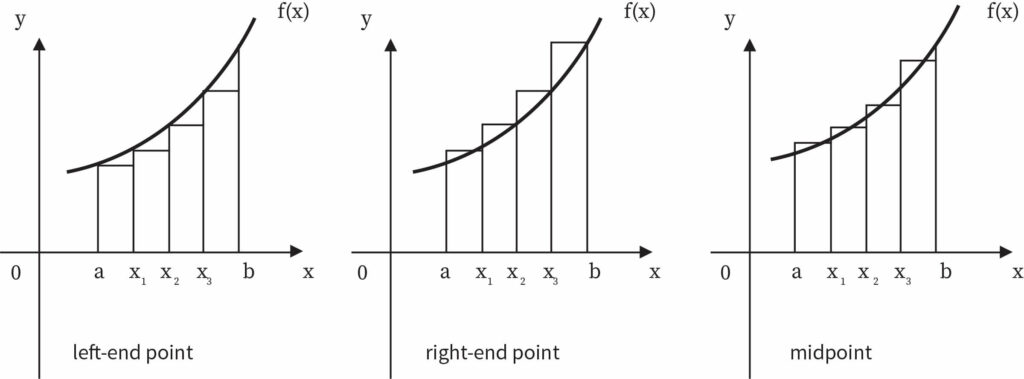
\includegraphics[width=\textwidth]{Example/assets/1.jpg}
\end{frame}

\begin{frame}{Fundamental theorem of calculus}
The fundamental theorem of calculus is a theorem that links the concept of differentiating a function with the concept of integrating a function. The two operations are inverses of each other apart from a constant value.

The first part of the theorem, the first fundamental theorem of calculus, states that for a function $f$, an antiderivative or indefinite integral $F$ may be obtained as the integral of $f$ over an interval with a variable upper bound. This implies the existence of antiderivatives for continuous functions.

Conversely, the second part of the theorem, the second fundamental theorem of calculus, states that the integral of a function $f$ over a fixed interval is equal to the change of any antiderivative $F$ between the ends of the interval. This greatly simplifies the calculation of a definite integral provided an antiderivative can be found by symbolic integration, thus avoiding numerical integration.
\end{frame}

\begin{frame}{Fundamental theorem of calculus}
    Let $f$ be a continuous real-valued function defined on a closed interval $[a, b]$. Let $F$ be the function defined, for all $x$ in $[a, b]$, by
$$
F(x)=\int_a^x f(t) d t .
$$
Then $F$ is uniformly continuous on $[a, b]$ and differentiable on the open interval $(a, b)$, and
$$
F^{\prime}(x)=f(x)
$$
for all $x$ in $(a, b)$ so $F$ is an antiderivative of $f$.
\end{frame}

\begin{frame}{Corollary}
The fundamental theorem is often employed to compute the definite integral of a function $f$ for which an antiderivative $F$ is known. Specifically, if $f$ is a real-valued continuous function on $[a, b]$ and $F$ is an antiderivative of $f$ in $[a, b]$ then
$$
\int_a^b f(t) d t=F(b)-F(a)
$$
\end{frame}

\begin{frame}{Mean value theorem}
    The fundamental theorem of calculus is proved using the mean value theorem, which states that:\\
    Let $f:[a, b] \rightarrow \mathbb{R}$ be a continuous function on the closed interval $[a, b]$, and differentiable on the open interval $(a, b)$, where $a<b$. Then there exists some $c$ in $(a, b)$ such that
$$
f^{\prime}(c)=\frac{f(b)-f(a)}{b-a} .
$$
\begin{center}
 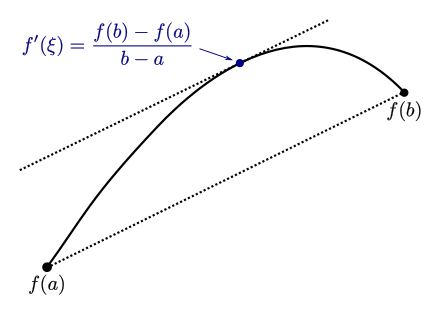
\includegraphics[width=0.4\textwidth]{Example/assets/2.png}   
\end{center}
\end{frame}

\begin{frame}{Definite Integral}
    Some of the MAT questions on calculus would be about computing the definite integral.
\end{frame}

\begin{frame}{Example 16}
What is the value of $\int_0^1\left(e^x-x\right)\left(e^x+x\right) \mathrm{d} x ?$\\
(a) $\frac{3 e^2-2}{6}$,\\
(b) $\frac{3 e^2+2}{6}$,\\
(c) $\frac{2 e^2-3}{6}$,\\
(d) $\frac{3 e^2-5}{6}$,\\
(e) $\frac{e^2+3}{6}$.
\end{frame}

\begin{frame}{Integration technique}
    There are some techniques we can apply to find the values of indefinite integrals:\\
    (a) Integration by substitution\\
    (b) Integration by part
\end{frame}

\begin{frame}{Comparing integrals}
Another common type of question on calculus is about comparing integrals.\\
There are some results we can use to help make comparisons without calculating the value of integrals:\\
\begin{itemize}
    \item $\int_a^b f(x) \mathrm{~d} x=-\int_b^a f(x) \mathrm{~d} x$
    \item $\int_a^b f(x) \mathrm{~d} x+\int_b^c f(x) \mathrm{~d} x=\int_a^c f(x) \mathrm{~d} x$
    \item if $f(x)>0$ for all $x\in [a,b]$, $\int_a^b f(x) \mathrm{~d} x>0$
    \item if $f(x)>g(x)$ for all $x\in [a,b]$, $\int_a^b f(x) \mathrm{~d} x>\int_a^b g(x) \mathrm{~d} x$
    \item if $m<f(x)<M$ for all $x \in [a,b]$, $(b-a)m<\int_a^b f(x) \mathrm{~d} x<(b-a)M$
\end{itemize}
Note: Always look out for special features (periodicity, upper/lower bound, zero, etc.) in the integrand.
\end{frame}

\begin{frame}{Example 17}
Which of these integrals has the largest value? You are not expected to calculate the exact value of any of these.\\
(a) $\int_0^2\left(x^2-4\right) \sin ^8(\pi x) \mathrm{d} x$\\
(b) $\int_0^{2 \pi}(2+\cos x)^3 \mathrm{~d} x$\\
(c) $\int_0^\pi \sin ^{100} x \mathrm{~d} x$\\
(d) $\int_0^\pi(3-\sin x)^6 \mathrm{~d} x$\\
(e) $\int_0^{8 \pi} 108\left(\sin ^3 x-1\right) \mathrm{d} x$\\
\end{frame}

\begin{frame}{Exercise 17}
Let
$$
f(x)=\int_0^1(x t)^2 \mathrm{~d} t, \quad \text { and } \quad g(x)=\int_0^x t^2 \mathrm{~d} t .
$$
Let $A>0$. Which of the following statements is true?\\
(a) $g(f(A))$ is always bigger than $f(g(A))$.\\
(b) $f(g(A))$ is always bigger than $g(f(A))$.\\
(c) They are always equal.\\
(d) $f(g(A))$ is bigger if $A<1$, and $g(f(A))$ is bigger if $A>1$.\\
(e) $g(f(A))$ is bigger if $A<1$ and $f(g(A))$ is bigger if $A>1$.
    
\end{frame}


\begin{frame}{Area under the curve}
\begin{columns}
    \begin{column}{0.5\textwidth}
    Integration is often used to find the area under the graph.\\
    A definite integral of a function can be represented as the signed area of the region bounded by its graph and the horizontal axis. In the above graph as an example, the integral of $f(x)$ is the blue $(+)$ area subtracted by the yellow $(-)$ area.
    \end{column}
    \begin{column}{0.5\textwidth}
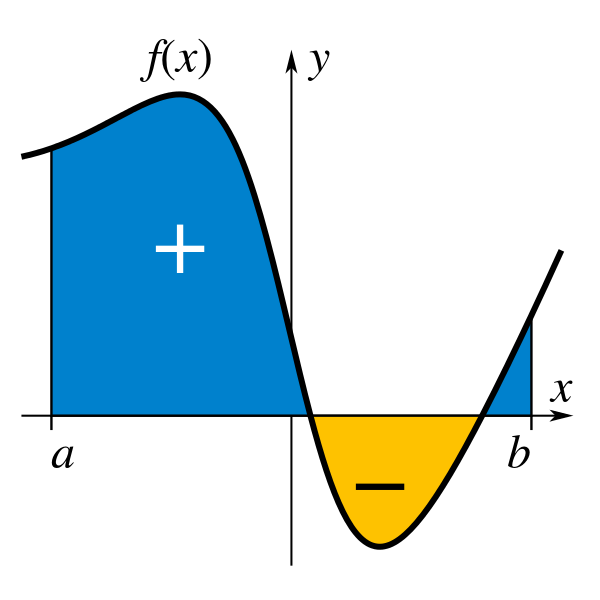
\includegraphics[width=\textwidth]{Example/assets/4.png}  
    \end{column}
\end{columns}
\end{frame}

\begin{frame}{Example 18}
Let $0<k<2$. Below is sketched a graph of $y=f_k(x)$ where $f_k(x)=x(x-k)(x-2)$. Let $A(k)$ denote the area of the shaded region.\\
\begin{center}
 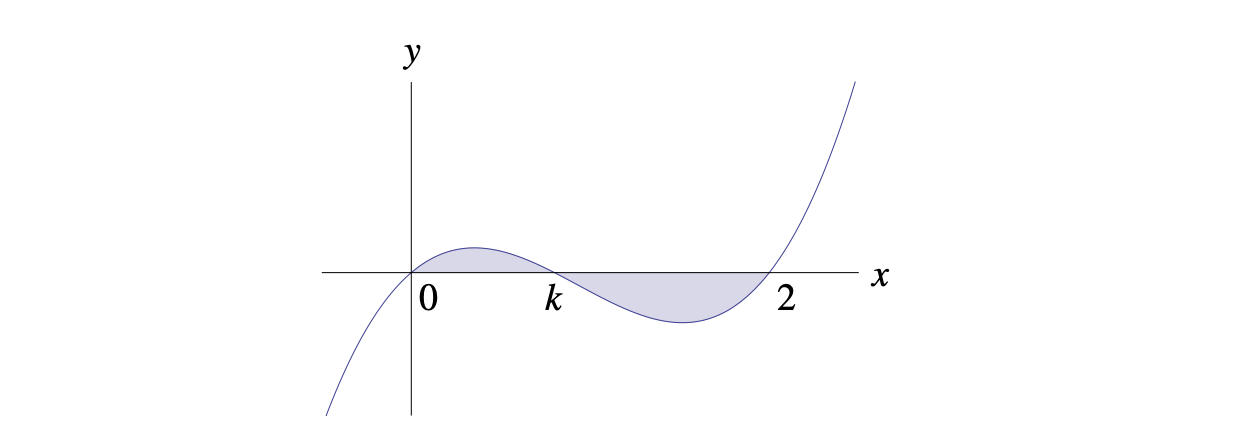
\includegraphics[width=0.7\textwidth]{Example/assets/3.png}   
\end{center}
(i) Without evaluating them, write down an expression for $A(k)$ in terms of two integrals.\\
(ii) Explain why $A(k)$ is a polynomial in $k$ of degree 4 or less. [You are not required to calculate $A(k)$ explicitly.]
\end{frame}

\begin{frame}{Example 18}
(iii) Verify that $f_k(1+t)=-f_{2-k}(1-t)$ for any $t$.\\
(iv) How can the graph of $y=f_k(x)$ be transformed to the graph of $y=f_{2-k}(x)$?\\
Deduce that $A(k)=A(2-k)$.\\
(v) Explain why there are constants $a, b, c$ such that
$$
A(k)=a(k-1)^4+b(k-1)^2+c .
$$
[You are not required to calculate $a, b, c$ explicitly.]
\end{frame}

\begin{frame}{Exercise 18}
A line is tangent to the parabola $y=x^2$ at the point $\left(a, a^2\right)$ where $a>0$. The area of the region bounded by the parabola, the tangent line, and the $x$-axis equals\\
(a) $\frac{a^2}{3}$,\\
(b) $\frac{2 a^2}{3}$,\\
(c) $\frac{a^3}{12}$,\\
(d) $\frac{5 a^3}{6}$,\\
(e) $\frac{a^4}{10}$. 
\end{frame}


\section{Numerical integration}
\begin{frame}{Riemann sum}
    Over or under estimation?\\
   If the graph is increasing on the interval, then the left-sum is an underestimate of the actual value and the right-sum is an overestimate.\\
   If the curve is decreasing, then the right-sum is an underestimate and the left-sum is an overestimate.\\
   In summary, it is judged by the monotonicity of the function.
\end{frame}

\begin{frame}{Trapezium rule}
    Generally speaking, the result obtained by the trapezium rule is $\frac{\text{right sum}+\text{left sum}}{2}$.\\
    \begin{columns}
        \begin{column}{0.5\textwidth}
            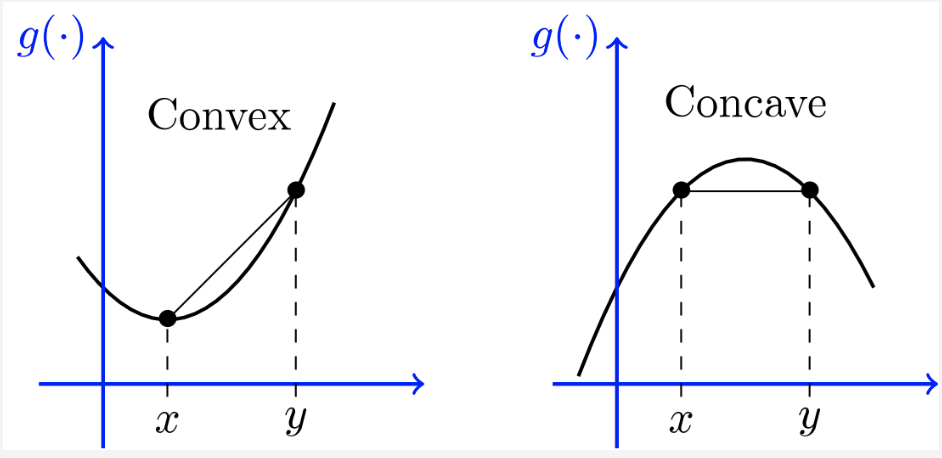
\includegraphics[width=\textwidth]{Example/assets/5.png}
        \end{column}
        \begin{column}{0.5\textwidth}
            The trapezoidal rule works by approximating the region under the graph of the function $f(x)$ as a trapezoid and calculating its area. It follows that
$$
\int_a^b f(x) d x \approx(b-a) \cdot \frac{1}{2}(f(a)+f(b)) .
$$
        \end{column}
    \end{columns}
\end{frame}

\begin{frame}{Trapezium rule}
The integral can be even better approximated by partitioning the integration interval. Let $\left\{x_k\right\}$ be a partition of $[a, b]$ such that $a=x_0<x_1<\cdots<x_{N-1}<x_N=b$ and $\Delta x_k$ be the length of the $k$-th subinterval (that is, $\Delta x_k=x_k-x_{k-1}$ ), then
$$
\int_a^b f(x) d x \approx \sum_{k=1}^N \frac{f\left(x_{k-1}\right)+f\left(x_k\right)}{2} \Delta x_k .
$$
When the partition has a regular spacing, as is often the case, that is, when all the $\Delta x_k$ have the same value $\Delta x$, the formula can be simplified for calculation efficiency by factoring $\Delta x$ out:
$$
\int_a^b f(x) d x \approx \frac{\Delta x}{2}\left(f\left(x_0\right)+2 f\left(x_1\right)+2 f\left(x_2\right)+2 f\left(x_3\right)+2 f\left(x_4\right)+\cdots+2 f\left(x_{N-1}\right)+f\left(x_N\right)\right)
$$ 
\end{frame}

\begin{frame}{Example 19}
When the trapezium rule is used to estimate the integral
$$
\int_0^1 2^x \mathrm{~d} x
$$
by dividing the interval $0 \leqslant x \leqslant 1$ into $N$ subintervals the answer achieved is\\
(a) $\frac{1}{2 N}\left\{1+\frac{1}{2^{1 / N}+1}\right\}$,\\
(b) $\frac{1}{2 N}\left\{1+\frac{2}{2^{1 / N}-1}\right\}$,\\
(c) $\frac{1}{N}\left\{1-\frac{1}{\left(2^{1 / N}-1\right)}\right\}$,\\
(d) $\frac{1}{2 N}\left\{\frac{5}{2^{1 / N}+1}-1\right\}$.
\end{frame}

\begin{frame}{Error}
     Over or under estimation?\\
   If the graph is concave-up/convex, the result obtained by the trapezium rule will be an over-estimation.\\
   If the curve is concave-down/concave, the result obtained by the trapezium rule will be an under-estimation.\\
   In summary, it is judged by the convexity (second derivative) of the function.
\end{frame}

\begin{frame}{Example 20}
If the trapezium rule is used to estimate the integral
$$
\int_0^1 f(x) \mathrm{d} x,
$$
by splitting the interval $0 \leqslant x \leqslant 1$ into 10 intervals then an overestimate of the integral is produced. It follows that\\
(a) the trapezium rule with 10 intervals underestimates $\int_0^1 2 f(x) \mathrm{d} x$;\\
(b) the trapezium rule with 10 intervals underestimates $\int_0^1(f(x)-1) \mathrm{d} x$;\\
(c) the trapezium rule with 10 intervals underestimates $\int_1^2 f(x-1) \mathrm{d} x$;\\
(d) the trapezium rule with 10 intervals underestimates $\int_0^1(1-f(x)) \mathrm{d} x$.
\end{frame}

\begin{frame}{Example 21}
The function $f(x)$ is defined for all real numbers and has the following properties, valid for all $x$ and $y$:\\
(A) $\quad f(x+y)=f(x) f(y)$.\\
(B) $\quad \mathrm{d} f / \mathrm{d} x=f(x)$.\\
(C) $\quad f(x)>0$.\\
Throughout this question, these should be the only properties of $f$ that you use; no marks will be awarded for any use of the exponential function.\\
Let $a=f(1)$.\\
(i) Show that $f(0)=1$.\\
(ii) Let
$$
I=\int_0^1 f(x) \mathrm{d} x
$$
Show that $I=a-1$.
\end{frame}

\begin{frame}{Example 21}
(iii) The trapezium rule with $n$ steps is used to produce an estimate $I_n$ for the integral I. Show that
$$
I_n=\frac{1}{2 n}\left(\frac{b+1}{b-1}\right)(a-1)
$$
where $b=f(1 / n)$.\\
(iv) Given that $I_n \geqslant I$ for all $n$, show that
$$
a \leqslant\left(1+\frac{2}{2 n-1}\right)^n
$$
    
\end{frame}

\begin{frame}{*Simpson's rule}
    One can improve further to use quadratics to estimate a definite integral.\\
    \begin{columns}
        \begin{column}{0.5\textwidth}
            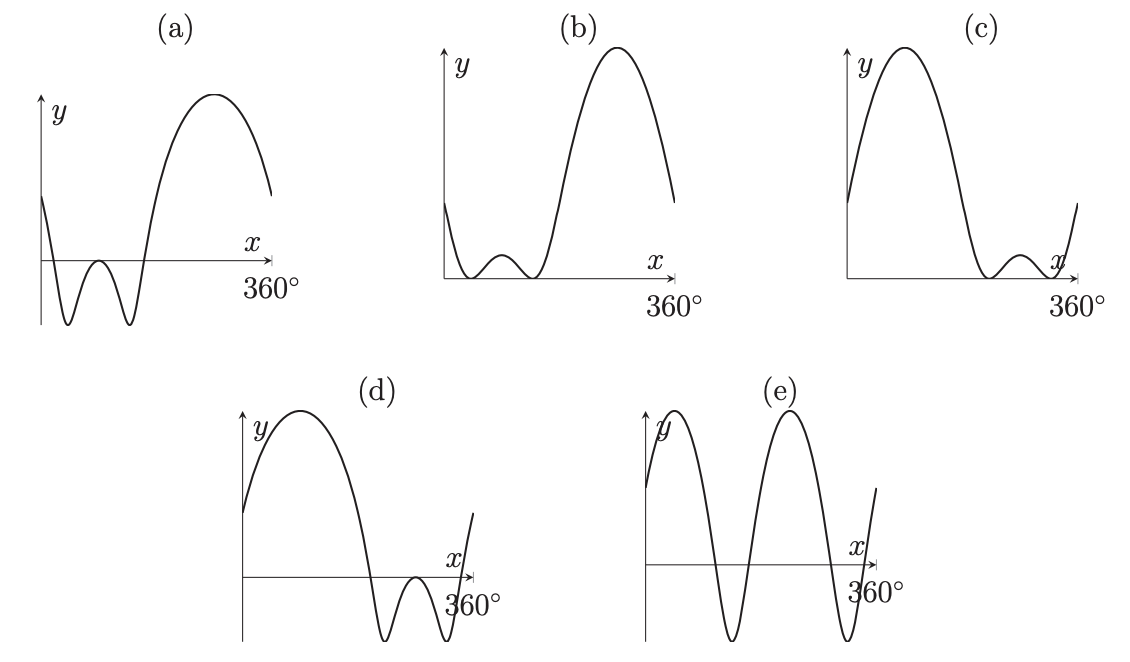
\includegraphics[width=0.7\textwidth]{Example/assets/6.png}
        \end{column}
        \begin{column}{0.5\textwidth}
            $\int_a^b f(x) d x \approx \frac{b-a}{6}\left[f(a)+4 f\left(\frac{a+b}{2}\right)+f(b)\right]$
        \end{column}
    \end{columns}
 Note: Simpson's rule will yield exact values when calculating definite integrals of polynomials of degree $3$ or less. Why?  
\end{frame}

\section{Differential equation}

\begin{frame}{General solution vs. particular solution}
    A solution of a differential equation is an expression for the dependent variable in terms of the independent one(s) which satisfies the relation. The general solution includes all possible solutions and typically includes arbitrary constants (in the case of an ODE) or arbitrary functions (in the case of a PDE.) A solution without arbitrary constants/functions is called a particular solution. Often we find a particular solution to a differential equation by giving extra conditions in the form of initial or boundary conditions.
\end{frame}

\begin{frame}{Example 22}
Show that $\cos c t$ and $\sin c t$ are solutions of the second order ODE
$$
\ddot{u}+c^2 u=0,
$$
where $c$ is a constant.
Deduce that $A \cos c t+B \sin c t$ is also a solution for arbitrary constants $A, B$.\\
Note: The solution $u=A \cos c t+B \sin c t$ contains two arbitrary constants and is the general solution of the second order ODE $\ddot{u}+c^2 u=0$. This illustrates the fact that the general solution of an $n$th order ODE contains $n$ arbitrary constants.
\end{frame}

\begin{frame}{Exercise 22}
The function $y=e^{k x}$ satisfies the equation
$$
\left(\frac{\mathrm{d}^2 y}{\mathrm{~d} x^2}+\frac{\mathrm{d} y}{\mathrm{~d} x}\right)\left(\frac{\mathrm{d} y}{\mathrm{~d} x}-y\right)=y \frac{\mathrm{d} y}{\mathrm{~d} x}
$$
for\\
(a) no values of $k$,\\
(b) exactly one value of $k$,\\
(c) exactly two distinct values of $k$,\\
(d) exactly three distinct values of $k$,\\
(e) infinitely many distinct values of $k$.
\end{frame}

\begin{frame}{Integral equation}
For all real numbers $x$, the function $f(x)$ satisfies
$$
6+f(x)=2 f(-x)+3 x^2\left(\int_{-1}^1 f(t) \mathrm{d} t\right) .
$$
It follows that $\int_{-1}^1 f(x) \mathrm{d} x$ equals\\
(a) 4,\\
(b) 6,\\
(c) 11,\\
(d) $\frac{27}{2}$,\\
(e) 23. 
\end{frame}

\begin{frame}{Example 23}
For a positive number $a$, let
$$
I(a)=\int_0^a\left(4-2^{x^2}\right) \mathrm{d} x .
$$
Then $\mathrm{d} I / \mathrm{d} a=0$ when $a$ equals\\
(a) $\frac{1+\sqrt{5}}{2}$,\\
(b) $\sqrt{2}$,\\
(c) $\frac{\sqrt{5}-1}{2}$,\\
(d) 1.
\end{frame}

\begin{frame}{Example 24}
Given a function $f(x)$, you are told that
$$
\begin{aligned}
\int_0^1 3 f(x) \mathrm{d} x+\int_1^2 2 f(x) \mathrm{d} x & =7 \\
\int_0^2 f(x) \mathrm{d} x+\int_1^2 f(x) \mathrm{d} x & =1 .
\end{aligned}
$$
It follows that $\int_0^2 f(x) \mathrm{d} x$ equals
(a) -1,\\
(b) 0,\\
(c) $\frac{1}{2}$,\\
(d) 2.
\end{frame}


\backmatter
\end{document}
